\chapter{Design Features and Implementation} % Main chapter title
\label{chap:Chapter4}  % For referencing the chapter elsewhere, use \ref{Chapter4}

\epigraph{”Our goals can only be reached through a vehicle of a plan, in which we must fervently believe, and upon which we must vigorously act. There is no other route to success." }{\textit{Pablo Picasso}}

% \epigraph{”Plan your work, execute it, get the result" }{\textit{ascertainsolo}}

Στο παρόν κεφάλαιο περιγράφεται η διαδικασία σχεδιασμού και υλοποίησης του \Abbr{MoCap} με χρήση drone swarm συστήματος, 
που συσχετίζεται η παρούσα διπλωματική. 

Μία high-level προσέγγιση, θα μπορούσε να διαχωρίζει το σύστημα σε τρία διακριτά
υποσυστήματα. Αρχικά το optical, του οποίου αρμοδιότητα είναι το detection, το tra\-cking, καθώς και η εκτίμηση
του range ή γωνίας του αντικειμένου από την camera. Δεύτερο, η λήψη των πληροφοριών από τους αισθητήρες ώστε να προσεγγιστεί η θέση του ίδιου
του drone. Τέλος, ο συνδυασμός των δύο παραπάνω μερών και η χρήση κατάλληλης localization τεχνικής για να βρεθεί η θέση του αντικειμένου
στο \Abbr{3D} χώρο.


%----------------------------------------------------------------------
\section{Equipment and Tools Used} \label{sec:design-tools}
Αρχικά θα αναφερθούν συνοπτικά η αρχιτεκτονική στην οποία έγινε επιλογή να επιλυθεί το πρόβλημα,
όπως επίσης και τα εξαρτήματα/αισθητήρια όργανα καθώς και τα λογισμικά τα οποία χρησιμοποιήθηκαν στην παρούσα διπλωματική. 

\subsection{Embedded Linux System}
Δύο πολύ δημοφιλείς επιλογές στον χώρο των ενσωματωμένων συστημάτων - ως κεντρικές μονάδες επεξεργασίας - είναι οι πλακέτες Raspberry Pi που κατασκευάζονται από την Raspberry Pi Foundation σε συνεργασία με την Broadcom, καθώς και οι πλακέτες Jetson της Nvidia. Στο \Fig{embedded-linux-systems} ως παράδειγμα παρουσιάζονται ενδεικτικά μία εκδοχή από την κάθε οικογένεια, ενώ στα \Tabl{raspberry-pi-specs} και \Tabl{jetson-nano-specs} τα τεχνικά χαρακτηριστικά της εκάστοτε πλακέτας ως αρχικό σημείο αναφοράς. 


\begin{figure} [H]
	\centering
	% -----------------
    \begin{minipage}{.5\textwidth}
      \centering
      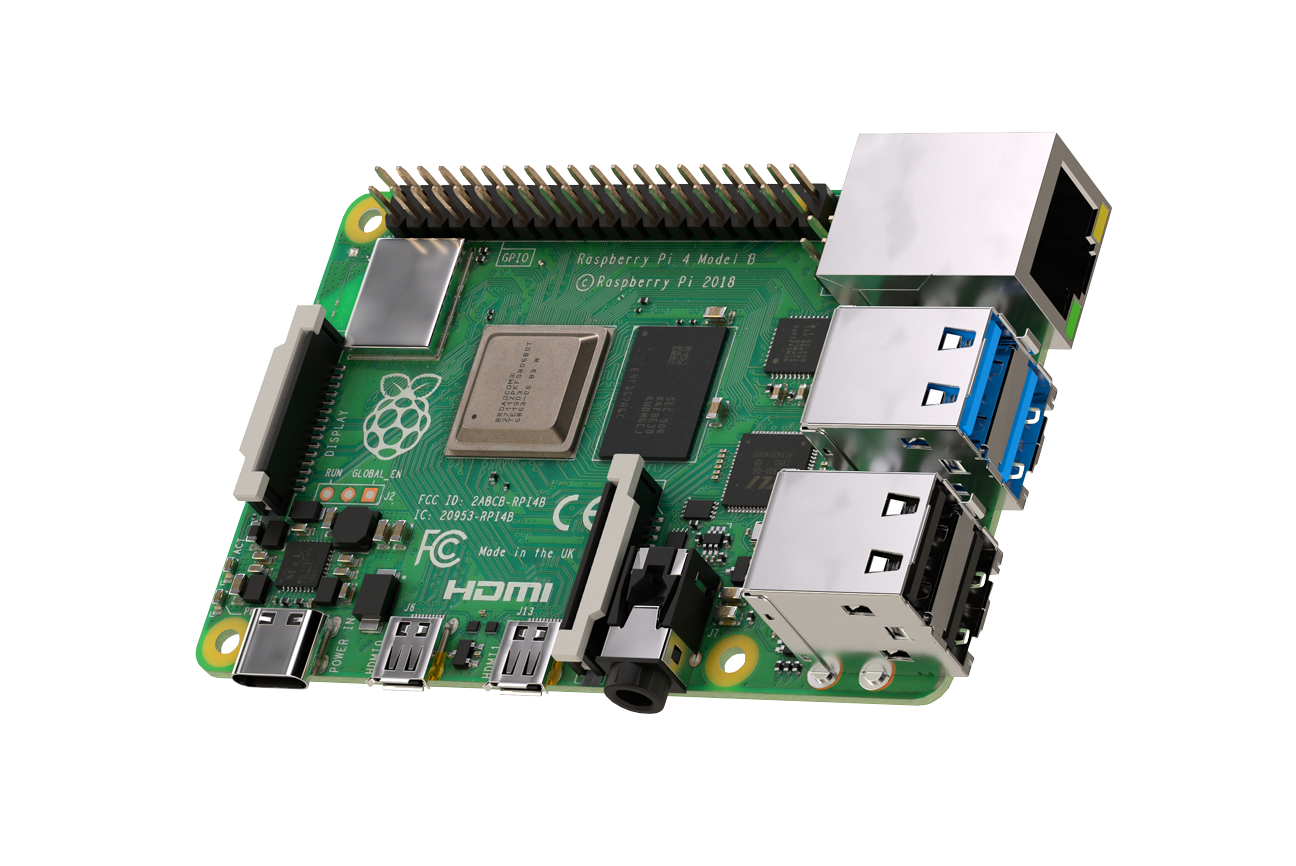
\includegraphics[width=\linewidth]{Images/Design-Implementation/raspberry-pi-4.png}\\
      {(a) Raspberry Pi 4 \URI{https://www.hellasdigital.gr/go-create/raspberry-and-accessories-el/raspberry-pi/raspberry-pi-4-4gb-ram/}}
    \end{minipage}%
    % -----------------
    \begin{minipage}{.5\textwidth}
      \centering
      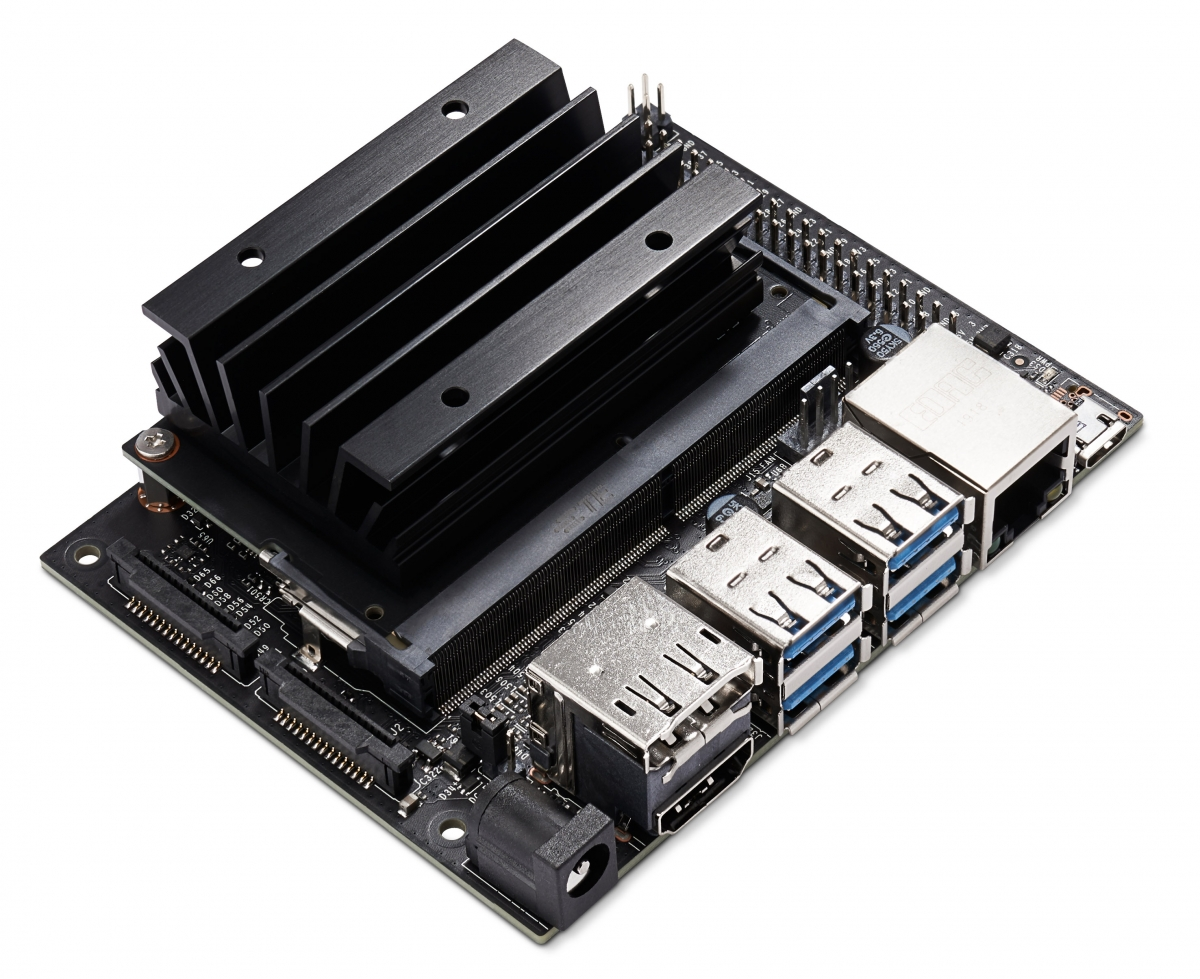
\includegraphics[width=.9\linewidth]{Images/Design-Implementation/jetson-nano.jpeg}\\
      {(b) Jetson Nano \URI{https://www.hellasdigital.gr/computers/accessories/nvidia-jetson-nano-developer-kit/}}
	\end{minipage}
	% -----------------
    \hfill \break
    \decoRule
    \CaptionBasedwithURL{Possible Embedded Linux Systems} 
    \label{fig:embedded-linux-systems}
\end{figure}

Και οι δύο επιλογές αποτελούνται από έναν ARM αρχιτεκτονικής Central Processing Unit (\Abbr{CPU}), ενώ στις Jetson βρίσκεται επιπρόσθετα και ένα Graphics Processing Unit (\Abbr{GPU}) που μπορεί να χρησιμοποιηθεί σε ενσωματωμένα με μεγάλες ανάγκες επεξεργασίας (όπως αυτά που σχετίζονται με εικόνα/βίντεο).

\begin{table}[H]
    \caption[]{Raspberry Pi 4 Model B Specifications}
    \label{tab:raspberry-pi-specs}
    \centering
    \resizebox{.6\textwidth}{!}{
        \begin{tabular}{ll}
            \hline
            \textbf{Feature} & \textbf{Value}  \\
            \hline
                Processor & \Centerstack{Broadcom BCM2711, Quad core Cortex-A72 \\(ARM v8) 64-bit SoC @ 1.5GHz }\\
                Memory & 8GB LPDDR4-3200 SDRAM \\
                Storage & External Micro-SD \\  
                Power & 5V DC (maximum 3A), 5-15Watt \\
                Cost & $\sim$100 €\\
                Weight & 46 grams (without case), 99 grams (with case) \\
                Peripherals & GPIO, I2C, SPI, UART \\
                \hline
        \end{tabular}
    }
  \end{table}

  Στην συγκεκριμένη διπλωματική επιλέχθηκε η ανάπτυξη του συστήματος να γίνει σε Raspberry Pi 4 boards - λόγω του ελάχιστα μικρότερου κόστους καθώς και μάζας τους - έχοντας μελλοντικά την επιλογή για migration ενός ή περισσότερων κόμβων του συστήματος σε Jetson boards, αν κριθεί αυτή η ανάγκη, για λόγους σχετικούς με την ταχύτερη επεξεργασία των δεδομένων.

  \begin{table}[H]
        \caption[]{Jetson Nano Developer Kit Specifications}
        \label{tab:jetson-nano-specs}
        \centering
        \resizebox{.6\textwidth}{!}{
            \begin{tabular}{ll}
                \hline
                \textbf{Feature} & \textbf{Value}  \\
                \hline
                    CPU & Quad-core ARM Cortex-A57 MPCore processor\\
                    GPU & \Centerstack{NVIDIA Maxwell architecture with 128 NVIDIA\\ CUDA® cores} \\
                    Memory & 4 GB 64-bit LPDDR4; 25.6 gigabytes/second \\
                    Storage & External Micro-SD \\  
                    Power & 5V DC, 5-10Watt \\
                    Cost & $\sim$120€\\
                    Weight & 250 grams (without case)\\
                    Peripherals & GPIO, I2C, I2S, SPI, UART \\
                    \hline
            \end{tabular}
        }
      \end{table}

% -----------------

\subsection{ROS}
Συνδετικός κρίκος των υποσυστημάτων είναι το open-source middleware Robot Operation System (\Abbr{ROS}) \cite{ros} το οποίο 
πε\-ρι\-λα\-μβά\-νει ένα εκτενές σύνολο εργαλείων, βιβλιοθηκών και συ\-μβά\-σεων. Τα πακέτα του οποίου χρησιμοποιούνται για την
λήψη και φιλτράρισμα από τους αισθητήρες των πληροφοριών, επικοινωνία μεταξύ των drone όπως τέλος και 
όποια τρι\-σδιά\-στα\-τη απεικόνιση χρειάζεται.

Μεγάλο πλεονέκτημα του \Abbr{ROS} είναι η ύπαρξη των packages. Τα packages είναι δια\-κρι\-τά αυτόνομα κομμάτια κώδικα τα οποία περικλείουν μία συχνά επαναλαμβανόμενη λογική, συνεπώς μπορούν να χρησιμοποιηθούν αυτούσια - με πολύ εύκολο τρόπο - σε διαφορετικές εφαρμογές χωρίς να υπάρχει η ανάγκη να κάνουμε \textit{reinvent the wheel} κάθε φορά, πετυχαίνοντας με αυτό τον τρόπο το rapid prototyping and testing ενός συστήματος καθώς και την αποφυγή δημιουργίας boilerplate κώδικα δίνοντας έμφαση περισσότερο στο main logic του εκάστοτε συστήματος. 

Το \Abbr{ROS} στην πραγματικότητα είναι ένα meta-operating system, με αποτέλεσμα να χρειάζεται να τρέχει σε ένα πρωτεύον Operating System (\Abbr{OS}), συγκεκριμένα μέχρι αυτήν την στιγμή απαιτεί την χρήση Ubuntu Linux. 

Στην συγκεκριμένη περίπτωση χρησιμοποιήθηκε η έκδοση noetic του \Abbr{ROS}, στην οποία εγκαταστάθηκαν τα παρακάτω πακέτα


ROS Packages(\TODO{update them}):
\begin{itemize}
  \addtolength{\itemindent}{0.3cm}
  \item tf2\_ros
  \item robot\_localization
  \item usb\_cam
  \item nmea\_navsat\_driver
\end{itemize}


% -----------------
\subsection{OpenCV}
Για το οπτικό σκέλος χρησιμοποιήθηκε η ανοιχτού κώδικα βιβλιοθήκη OpenCV \cite{opencv}, η οποία αποτελεί την δημοφιλέστερη επιλογή για real-time Computer Vision related εφαρμογές. Ξεκίνησε η ανάπτυξη της στα εργαστήρια της Intel και έχει ήδη διάρκεια ζωής λίγο περισσότερο από δύο δεκαετίες. Για τις ανάγκες στης συγκεκριμένης εργασίας χρησιμοποιήθηκε η έκδοση της \TODO{add opencv version}.

% -----------------
\subsection{Camera}
Σχετικά με την κάμερα, ήταν ανάγκη - όντας πρώτη γενιά του συστήματος -  να επιλεχθεί μία low-cost 1080p camera η οποία θα παρέχει δυνατότητα επιλογής χαμηλότερου resolution για λόγους δοκιμών. Στο πρωτότυπο σύστημα τελικά γίνεται χρήση μία 1080p web cameras της Creative \cite{creative-camera} - \Fig{creative-camera} - με δυνατότητες λήξης βίντεο στα 30fps, η οποία συνδέεται μέσω USB στο Raspberry Pi.

\FigCaptLabelBasedURL{Images/Design-Implementation/creative-web-cam.jpeg}%
{Camera used for ball detection and tracking}%
{creative-camera}%
<0.4>%
(https://en.creative.com/p/peripherals/creative-live-cam-sync-1080p)


% -----------------
\subsection{GPS}
Παρόλο που - όπως αναφέρθηκε στο \Chap{thesis-approach} - στο συγκεκριμένο σύστημα μας ενδιαφέρει το relative positioning και όχι το absolute, σκεπτόμενοι ότι στην πραγματικότητα το σύστημα σχεδιάζεται με γνώμονα το να λειτουργεί σε outdoor scenarios\udot ένας άμεσος τρόπος προσδιορισμού της θέσης του κάθε drone είναι με χρήση κάποιου εμπορικού αισθητήρα \Abbr{GPS}. Στην συνέχεια και αφού έχει αποκτηθεί πληροφορία απόλυτης θέσης για το κάθε drone μπορεί - θεωρώντας ένα από αυτά ως αρχή των αξόνων - να γίνει translate των απόλυτων συντεταγμένων ώστε να κρατηθεί μόνο πληροφορία σχετικά με την χωρική τοπολογία του δικτύου.

Συγκεκριμένα, χρησιμοποιείται το GPS για commercial χρήση ΒΝ-220 \cite{bn-220-gps}, το οποίο υπόσχεται εμβέλειας ακρίβειας της τάξης των δύο μέτρων. Πρακτικά, παρόλο που για ένα \Abbr{MoCap} σύστημα αυτή η τιμή είναι απαγορευτική, χρησιμοποιείται στα πρώτα versions, καθαρά αναφορικά με την εξικοίωση του τρόπου επικοινωνίας \Abbr{ROS} - \Abbr{GPS}. Σε επόμενα revisions σκοπός είναι η αντικατάσταση του με \Abbr{RTK}-\Abbr{GPS} που συχνά μπορεί να φέρουν drone για αυτήν την χρήση\footnote{Τα drone του εργαστηρίου SenseLab, } ώστε να φτάσει η συνολική ακρίβεια εκτίμησης της απόλυτης θέσης στα μερικά εκατοστά. 

Το συγκεκριμένο GPS συνδέεται με το Raspberry Pi μέσω Universal Asynchronous Receiver-Transmitter (\Abbr{UART}) \TODO{add cite} σύνδεσης και χρησιμοποιεί NMEA \TODO{add cite} πακέτα για την επικοινωνία. 

\FigCaptLabelBasedURL{Images/Design-Implementation/bn220.png}%
{GPS module used to estimate position}%
{bn-220-gps}%
<0.4>

% -----------------
\subsection{IMU}
\cite{adafruit-10dof-imu}
\FigCaptLabelBasedURL{Images/Design-Implementation/10DoF-Adafruit-IMU.jpeg}%
{Adafruit 10 DoF IMU}%
{adafruit-10DoF-imu}%
<0.4>

% -----------------
\subsection{Breakout Board}
Για να λειτουργήσουν τα παραπάνω υποσυστήματα, χρειαζόταν να πραγματοποιηθούν οι κατάλληλες συνδέσεις μεταξύ τους. Η απλούστερη εκδοχή θα ήταν να γίνει αυτό με χρήση breadboard, πράγμα όμως που θα πρόσθετε όγκο και βάρος στο τελικό σύστημα, τα οποία σε περίπτωση δοκιμών πάνω σε πραγματικά drone θα ήταν απαγορευτικοί παράγοντες όμως. Συνεπώς, προκειμένου να μπορεί με ευκολία να γίνει η ανάπτυξη του συστήματος, σχεδιάστηκε (στο cad εργαλείο KiCad \cite{KiCad}) και κατασκευάστηκε ένα custom breakout, το οποίο παρέχει εύκολη πρόσβαση στα GPIO του Raspberry, έξτρα pins για τροφοδοσία στα 5 και 3.3 Volt, pins για τοποθέτηση αισθητήρων - όπως του \Abbr{IMU} - καθώς και mounting holes στα οποία μπορεί να τοποθετηθεί 40x40mm fan για την ψύξη του συστήματος. 

% Image
\FigCaptLabelBasedURL{Images/Design-Implementation/Rpi-breakout.png}%
{Raspberry Pi breakout}%
{raspberry-pi-breakout}%
<0.55>

\cite{raspberry-pi-fan-breadkout}


% -----------------
\subsection{System Overview}

% Image
\FigCaptLabelBasedURL{Images/Design-Implementation/thesis-system.jpg}
{System designed}%
{thesis-system}%
<0.65>

\begin{table}[H]
    \caption[]{Bill of Materials}
    \label{tab:thesis-system-bom}
    \centering
    \resizebox{0.6\textwidth}{!}{
        \begin{tabular}{ll}
            \hline
            \textbf{Component} & \textbf{Cost}  \\
            \hline
                Raspberry Pi 4 Model B 8GB & \Centerstack{$\sim$ 100 €}\\
                Creative live cam sync 1080p \cite{creative-camera} & \Centerstack{$\sim$ 44 €}\\
                Adafruit 10 DoF IMU \cite{adafruit-10dof-imu} & \Centerstack{$\sim$ 30 €}\\
                BN-220 GPS Module \cite{bn-220-gps} & \Centerstack{$\sim$ 15 €}\\
                Breakout Board with fan \cite{raspberry-pi-fan-breadkout} & \Centerstack{$\sim$ 8 €}\\
                \hline
        \end{tabular}
    }
  \end{table}


% ------------------------------------------------------------------------------------------------------
\section{Environment}
\subsection{Operation System} 
\subsection{Sensors' Communication} 


\begin{lstlisting}[language=sh, escapechar=@, caption={Descriptive Caption Text},label=DescriptiveLabel]
    @\color{dkgreen}{\$}@ sudo apt-get update
\end{lstlisting}


%----------------------------------------------------------------------
\section{Camera}
Internal parameters
    Intrinsic 
    Distortion (ideal Pinhole model does not have lens)

    
Extrinsic 
\subsubsection{Camera Calibration}
\subsubsection{Ball Detection and Tracking}
\subsubsection{Range Estimation}

%----------------------------------------------------------------------

\section{Networking}

%----------------------------------------------------------------------

